\vspace{-1\baselineskip}

\begin{problemAllDefault}{Купе}

\mytextandpicture{Купейний вагон містить 36 пасажирських місць\nolinebreak[3] --- 9~купе по 4 місця у кожному. Половина серед цих місць нижні, решта --- верхні. На рисунку наведено схему розміщення місць 1, 2, 3, 4 у купе \textnumero$\,$1. Купе \textnumero$\,$2 містить аналогічно розміщені місця 5, 6, 7, 8, і так далі, до купе \textnumero$\,$9, яке містить аналогічно розміщені місця 33, 34, 35, 36.}{\begin{minipage}{4.5cm}\vbox to 4\baselineskip{\vss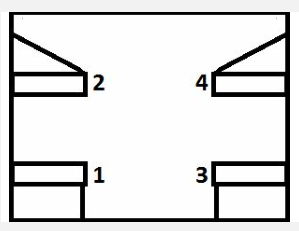
\includegraphics[width=4.5cm]{Kupe.pdf}}\end{minipage}}

% % % Купейний вагон містить 36 пасажирських місць\nolinebreak[3] --- 9~купе по 4 місця у кожному. Половина серед цих місць нижні, решта --- верхні. На рисунку наведено схему розміщення місць 1, 2, 3, 4 у купе №1. Купе №2 містить аналогічно розміщені місця 5, 6, 7, 8, і так далі, до купе №9, яке містить аналогічно розміщені місця 33, 34, 35, 36.

\ifAfour
\vspace{-0.5\baselineskip}
\else
\vspace{0.5\baselineskip}
\fi

% % % %%% \myflfigaw{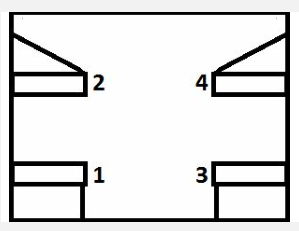
\includegraphics[width=4.75cm]{Kupe.pdf}}
% % % \mytextandpicture{
Напишіть програму, яка, прочитавши номери двох різних місць одного купейного вагону, визначатиме:
\begin{enumerate}
\item
чи в одному й тому ж купе розміщені ці місця;
\item
верхнє чи нижнє перше з цих місць;
\item
верхнє чи нижнє друге з цих місць.
\end{enumerate} % % % }{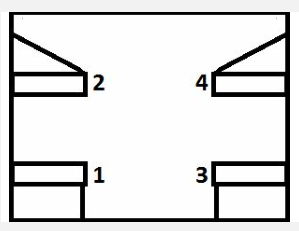
\includegraphics[width=4.875cm]{Kupe.pdf}}

\InputFile Два числа $p_1\,\,\,p_2$ у одному рядку, розділені одним пропуском (пробілом). Гарантовано виконуються обмеження ${1\,{\<}\,p_1\,{\<}\,36}$, ${1\,{\<}\,p_2\,{\<}\,36}$, ${p_1\,{\neq}\,p_2}$.

\OutputFile Перший рядок повинен містити або єдине слово \texttt{NO} (якщо місця у різних купе), або слово \texttt{YES} і після нього через пробіл номер того купе, в якому розміщені обидва ці місця. Другий рядок повинен містити або єдине слово \texttt{LOW} (якщо перше з уведених місць нижнє), або єдине слово \texttt{HIGH} (якщо верхнє). Третій рядок теж повинен містити або слово \texttt{LOW}, або слово \texttt{HIGH}, але стосовно другого з уведених місць.

\Examples
\begin{exampleSimple}{3em}{3em}%
\exmp{2 3}{YES 1
HIGH
LOW}%
\end{exampleSimple}
\begin{exampleSimple}{3em}{3em}%
\exmp{23 17}{NO
LOW
LOW}%
\end{exampleSimple}

\Note
Перевірте правильність написання у Вашій програмі слів \texttt{YES}, \texttt{NO}, \texttt{LOW}, \texttt{HIGH} (ВЕЛИКИМИ латинськими літерами). Автоматична перевіряюча система зараховує відповідь, лише коли вона правильна буква-в-букву.

\end{problemAllDefault}
